\documentclass{article}
\usepackage{amsmath, mathtools, amsfonts, amssymb, bm}
\usepackage{tikz, pgf}

\begin{document}
\textbf{Abhinaash Tiwari Roll no: 22}
\textbf{ASSIGNMENT I - MATH 101 - 2022}

\textit{KATHMANDU UNIVERSITY DEPARTMENT OF MATHEMATICS}

\begin{enumerate}
\item Find the domain and range of each function.
	\begin{enumerate}
		\item $f(x) = 1 + x^2$
		\item $f(x) = 1 - \sqrt{x}$
		\item $f(z) = \sqrt{4 - z^2}$
		\item $f(t) = \frac{1}{1 + \sqrt{t}}$
	\end{enumerate}
\item \textbf{What symmetries, if any, do the graphs have?}

(a) $y = -x^2$

(b) $y = -\frac{1}{x}$

(c) $y = \frac{p}{|x|}$

(d) $y = (-x)^{3/2}$
\item Determine whether the function is even, odd, or neither.
\begin{enumerate}
\item $f(x) = 3$
\item $f(x) = x^3 + x$
\item $f(x) = \frac{1}{x^2 + x + 1}$
\end{enumerate}
\item Find domain and ranges of f, g, f + g, f.g.
\begin{enumerate}
\item $f(x) = x$, $g(x) = \sqrt{x - 1}$
\item $f(x) = \sqrt{x + 1}$, $g(x) = \sqrt{x - 1}$
\end{enumerate}
\item{Find domain and ranges of f/g and g/f}

If $f(x) = 2$ and $g(x) = x^2 + 1$, then
\begin{align*}
\frac{f(x)}{g(x)} &= \frac{2}{x^2 + 1} \\
\frac{g(x)}{f(x)} &= \frac{x^2 + 1}{2}
\end{align*}

\item \textbf{Graph the functions:}

(a) $f(x) = 
\begin{cases}
x & 0 \leq x \leq 1 \\
2 - x & 1 < x \leq 2
\end{cases}$

(b) $g(x) = 
\begin{cases}
\frac{1}{x} & x < 0 \\
x & 0 \leq x
\end{cases}$

\item\begin{enumerate}
\item What real numbers satisfy the equation $bxc = dxe$?
\item Does $d - xe = -bxc$? Give reasons for your answer.
\end{enumerate}
\item \textbf{Match the equations listed (a) - (d) to the graphs in the given figure.}

(a) $y = (x - 1)^2 - 4$

(b) $y = (x - 2)^2 + 2$

(c) $y = (x + 2)^2 + 2$

(d) $y = (x + 3)^2 - 2$

\begin{figure}
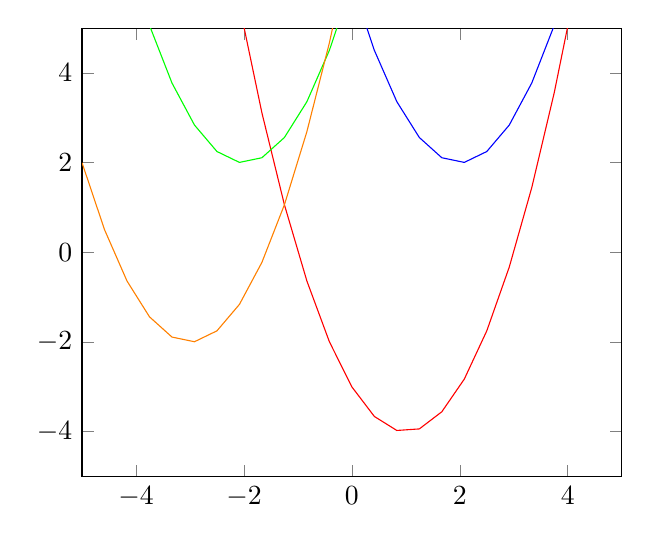
\begin{tikzpicture}
\begin{axis}[xmin=-5,xmax=5,ymin=-5,ymax=5]
\addplot[color=red]{(x - 1)^2 - 4};
\addplot[color=blue]{(x - 2)^2 + 2};
\addplot[color=green]{(x + 2)^2 + 2};
\addplot[color=orange]{(x + 3)^2 - 2};
\end{axis}
\end{tikzpicture}
\end{figure}


\item Define the following and graph it (at least one graph).
\begin{enumerate}
\item Quadratic function
\item Exponential and Logarithmic functions
\item Circle, Parabola, Ellipse and Hyperbola
\end{enumerate}

\item \textbf{Evaluate the following limits:}

(a) $\lim_{x \to 2} \frac{x - \sqrt{8 - x^2}}{\sqrt{x^2 + 12 - 4}}$

(b) $\lim_{x \to 4} \frac{4x - x^2}{2 - \sqrt{x}}$

(c) $\lim_{x \to \infty} \frac{x + \sin x}{x + \cos x}$

(d) $\lim_{x \to -1} \frac{\sqrt{x^2 + 8 - 3}}{x + 1}$

(e) $\lim_{x \to 1-} \frac{\sqrt{2x(x - 1)}}{|x - 1|}$

(f) $\lim_{x \to -2+} \frac{(x - 3)|x + 2|}{x + 2}$


(g) $\lim_{x \to -2-} \frac{(x - 3)|x + 2|}{x + 2}$

(h) $\lim_{t \to 4+} \frac{|t|}{t}$

(i) $\lim_{x \to 4-} \frac{|x|}{x}$

(j) $\lim_{x \to \infty} \left(\sqrt{x} - \sqrt{x - 3}\right)$

(k) $\lim_{x \to 0} \frac{\sin x - x}{x^3}$

(l) $\lim_{x \to 1} \frac{x - 1}{\ln x - \sin \pi x}$

(m) $\lim_{x \to \infty} \frac{\sqrt{3} x - \sqrt{5} x}{\sqrt{3} x + \sqrt{5} x}$

(n) $\lim_{\theta \to 3-} \frac{d\theta}{e^{\theta}}$

\item \textbf{Find the limits:}

(a) $\lim_{x \to 0+} \frac{2}{\sqrt{x^2 + 3}}$

(b) $\lim_{x \to \pi} \frac{2}{-\tan x}$

(c) $\lim_{t \to \infty} \frac{2 - t + \sin t}{t + \cos t}$

(d) $\lim_{x \to \pi} \frac{2}{\sec x}$

\item \textbf{State Sandwich Theorem and use it to find the following limits:}

(a) Show that if $\lim_{x \to c} |f(x)| = 0$, then $\lim_{x \to c} f(x) = 0$.

(b) If $\sqrt{2 - x^2} \le f(x) \le 2 \cos x$ for all $x$, find $\lim_{x \to 0} f(x)$.

(c) If $1 - \frac{x^2}{6} < \frac{x \sin x}{2 - 2 \cos x} < 1$ for all $x$, find $\lim_{x \to 0} \frac{x \sin x}{2 - 2 \cos x}$.

\item \textbf{State the $\epsilon - \delta$ definition of limit for the function $f(x)$ at $x = c$. Find $\delta > 0$.}

(a) $f(x) = x + 1$, $x_0 = 4$, $\epsilon = 0.01$.

(b) $\lim_{x \to 1} f(x) = 1$, if $f(x) = 
\begin{cases}
x^2 & \text{if } x \neq 1 \\
2 & \text{if } x = 1
\end{cases}$

(c) $f(x) = \sqrt{1 - 5x}$, $x_0 = -3$, $\epsilon = 0.5$.

\item \textbf{Evaluate:}

(a) $\lim_{x \to \frac{\pi}{2}} \frac{\tan x}{\frac{\pi}{2} - x}$

(b) $\lim_{x \to 1^+} \frac{(x - 1)^{\frac{1}{1-x}}}{x}$

(c) $\lim_{x \to 0^+} \frac{(1 + x)^{\frac{1}{x}}}{1}$

(d) $\lim_{x \to 0} \frac{\cos x - e}{x \sin x}$

(e) $\lim_{x \to 0} \frac{\frac{1}{x} - \frac{1}{\sin x}}{1}$

(f) $\lim_{x \to \infty} \frac{x \sin \frac{1}{x}}{x}$

(g) $\lim_{x \to 0} \frac{\frac{3}{x - 1}}{\frac{2}{x - 1}}$

(h) $\lim_{x \to 0} \frac{a}{\frac{x - b}{x}}$

(i) $\lim_{x \to 0} \frac{\ln(5 + x) - \ln(5 - x)}{x}$

(j) $\lim_{x \to 0} \frac{x - \sin^{-1} x}{\frac{x^3}{3}}$

(k) $\lim_{x \to \frac{\pi}{2}} \frac{\sin x}{\tan x}$

(l) $\lim_{\theta \to \frac{\pi}{2}} \frac{1 - \cos \theta}{1 + \cos 2\theta}$

(m) $\lim_{x \to 0} \frac{\cos x - 1}{x}$

(n) $\lim_{x \to 0} \frac{\ln x - 1}{x - e}$

(o) $\lim_{x \to 0} \frac{\frac{2 + x}{2 - x}}{\frac{1}{x}}$

(p) $\lim_{x \to \infty} \frac{\frac{x + 2}{x - 1}}{\frac{1}{x}}$

(q) $\lim_{x \to \infty} \frac{\frac{x + 2}{x - 1}}{x}$

(r) $\lim_{x \to 0^+} \frac{\sin x \ln x}{x}$

(s) $\lim_{x \to \infty} \frac{\log_2 x}{\log_3 (x + 3)}$

(t) $\lim_{x \to \infty} \frac{\ln x}{\frac{1}{x}}$

(u) $\lim_{x \to 0} \frac{e^{\frac{x + x}{2}}}{\frac{1}{x}}$


\item \textbf{State the condition for the existence of the limit of a function at a point. Given that:}

\[f(x) =\begin{cases}3 - x & x < 2 \\3 & x = 2 \\\frac{x^2 + 1}{x} & x > 2\end{cases}\]

\textbf{Does the limit} $\lim_{x \to 2} f(x)$ \textbf{exist? If yes, what is its value? If no, why isn’t?}

\item \textbf{What does it mean for a function to be right continuous at a point? and left continuous at a point? How the continuity and one - sided continuity related?}

\[f(x) =
\begin{cases}
1 & \text{when } x \leq -1 \\
-x & \text{when } 0 < x < 0 \\
1 & \text{when } x = 0 \\
-x & \text{when } 0 < x < 1 \\
1 & \text{when } x \geq 1
\end{cases}\]

\textbf{Examine limits, continuity and one sided continuity of f at each of the points x =} -1, 0, 1.

\item \textbf{For what value of a is the function}
\begin{enumerate}
    \item[(a)] $f(x) = 
    \begin{cases}
        \frac{x^2 - 1}{2} & \text{if } x < 3 \\
        2ax & \text{if } x \geq 3
    \end{cases}$ \textbf{continuous at every x.}
    \item[(b)] $f(x) = 
    \begin{cases}
        x^2 & \text{if } x < 3 \\
        4ax^3 - 1 & \text{if } x \geq 3
    \end{cases}$ \textbf{continuous at every x.}
\end{enumerate}

\item \textbf{Define the discontinuity of a function at a point. Discuss the types of discontinuity with examples. Also find the continuous extension of}
\begin{enumerate}
    \item[(a)] $f(x) = \frac{x^2 + x - 6}{x^2 - 4}$ \textbf{at point x = 2.}
    \item[(b)] $f(x) = \frac{x^2 - 16}{x^2 - 3x - 4}$ \textbf{at point x = 4.}
\end{enumerate}
 \item \textbf{(a) Let } $f(x) = 
\begin{cases}
    \frac{x^2}{\sin \frac{1}{x}} & \text{if } x < 0 \\
    \sqrt{x} & \text{if } x \geq 0
\end{cases}$ \textbf{be a function. Find } $\lim\limits_{x \to 0^+} f(x)$ \textbf{and } $\lim\limits_{x \to 0^-} f(x)$.

\textbf{Can anything be said about } $\lim\limits_{x \to 0} f(x)$ \textbf{?}

\textbf{(b) If } $f(x) = 
\begin{cases}
    x \sin \frac{1}{x} & \text{if } x \neq 0 \\
    0 & \text{if } x = 0
\end{cases}$ \textbf{. Does the function continuous at x = 0?}

\item \textbf{At which points do the following functions fail to be continuous?}

(a) $y = \frac{1}{(x + 2)^2 + 4}$

(b) $y = \frac{x + 1}{x^2 - 4x + 3}$

(c) $y = \frac{x^2 - 16}{x^2 - 3x - 4}$

(d) $y = \frac{x + 2}{\cos x}$

\item Examine the continuity of the functions.
(a) f(x) =
\begin{cases}
x & \text{for } 0 < x < 1 \
2 - x & \text{for } 1 \leq x \leq 2 \
\frac{x - 2}{2} & \text{for } x > 2
\end{cases}

at x = 1 and x = 2.

(b) f(x) =
\begin{cases}
\sin(2x) + 1 & \text{for } -\frac{\pi}{2} \leq x < 0 \
e^{2x} & \text{for } 0 \leq x < \frac{\pi}{2} \
e^{2x} \cos x & \text{for } x \geq \frac{\pi}{2}
\end{cases}

at x = 0 and x = $\frac{\pi}{2}$.

\item Show that the function $f(x) = \begin{cases} \sin^2 \frac{ax}{x} & x \neq 0 \ 1 & x = 0 \end{cases}$ is discontinuous at $x=0$. Redefine the function in such a way that it becomes continuous at $x=0$.
\item Show that $3^x$ grows faster than $2^x$.
\item Show that $\sqrt{x^2 + 5}$ and $(2\sqrt{x} - 1)^2$ grow at the same rate.
 
\item Find the slope, the equation of the tangent, and the equation of the normal to the following curves at the given point:

(a) $x^2 + xy - y^2 = 1$ at $(2, 3)$

(b) $x \sin 2y = y \cos 2x$ at $(\frac{\pi}{4}, \frac{\pi}{2})$

(c) $x^2 \cos 2x - \sin y = 0$ at $(0, \pi)$

(d) $y = e^x + 2$ at $(0, 2)$

\item Does the curve $y = x^4 - 2x^2 + 2$ have any horizontal tangents? If yes, where?
\item Find the two points where the curve $x^2 + xy + y^2 = 7$ crosses the $x$-axis. Show that the tangents to the curve at these points are parallel. What is the common slope of these tangents?

\item Find the points on the curve $x^2 + xy + y^2 = 7$, where the tangent is parallel to the $x$-axis and where the tangent is parallel to the $y$-axis.

\item The curve $y = ax^2 + bx + c$ passes through the point $(1, 2)$ and is tangent to the line $y = x$ at the origin. Find $a$, $b$, and $c$.

\item The curves $y = x^2 + ax + b$ and $y = cx - x^2$ have a common tangent to the line at the point $(1, 0)$. Find $a$, $b$, and $c$.










\end{enumerate}
\end{document}

